
\title{Gerenciamento de memória}

\frame{\titlepage}

\begin{frame}
\frametitle{Revis\~ao: processos}

 \begin{block}{Visão geral}
        \begin{itemize}
        \item Composto por código do programa em execução, arquivos
          abertos, sinais pendentes, dados internos do núcleo do SO,
          estado do processador, espaço de endereço, uma ou mais {\em
            threads} de execução, seção de dados contendo variáveis globais;
            \item \textit{Threads};
          \item Escalonamento;
          \item Sincronização;
          \item Comunicação entre processos.
           
        \end{itemize}
      \end{block}

\end{frame}

\begin{frame}{Divisão do curso}
  \footnotesize
  O curso será dividido em $3$ tópicos principais envolvendo
  Gerenciamento de:
  \begin{enumerate}
  \item Processos;
  \item {\large\alert{Memória}};
  \item Entrada e saída (E/S).
  \end{enumerate}
%    \includegraphics[scale=0.55]{intro_computer_system-modules.pdf}
\end{frame}

\section{Hierarquia de memória}

\def\headcolor{blue!80!black}

\begin{frame}
\frametitle{Custo e proximidade do processador
\footnote{\scriptsize Computer Architecture. 
Patterson and Hennessy. Morgan-Kaufmann, 5th edition 2012.}}
\small  
  \begin{tabular}[h]{c|c|c} \hline
    \color{\headcolor}{Tecnologia} &  \color{\headcolor}{Tempo de acesso (ns)} &  \color{\headcolor}{US\$ por GB (2012)}\\ \hline
    SRAM semi-condutora & 0,5--2,5 & \$500--\$1000\\
    DRAM semi-condutora& 50-70 & \$10--\$20\\
    Flash semi-condutora& 5.000-50.000 & \$0,75--\$1\\
    Disco magnético & 5.000.000 -- 20.000.000 & \$0.05-\$0,10\\ \hline
  \end{tabular}
  
\end{frame}

\begin{frame}{Hierarquia de memória}

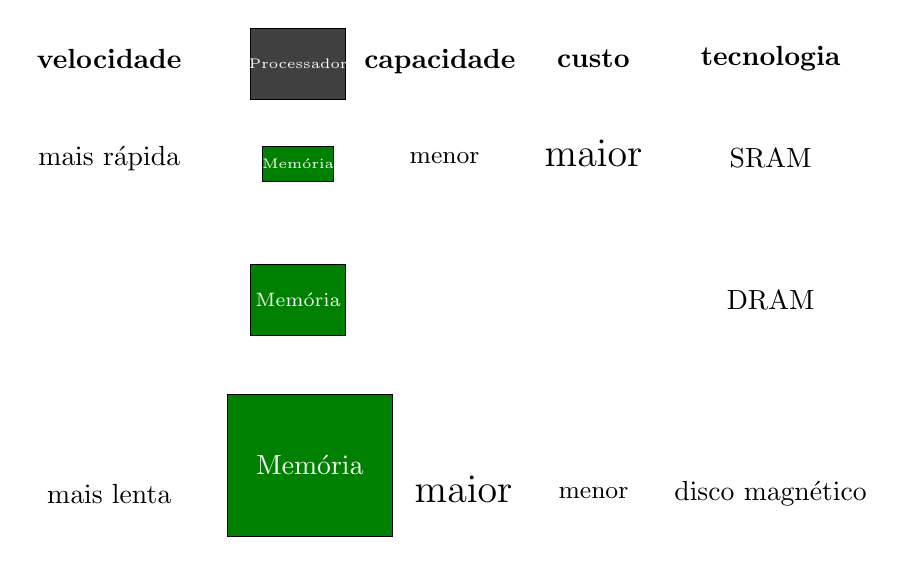
\begin{tikzpicture}[scale=0.6,head/.style={color=purple,anchor=center},
  labelsty/.style={anchor=center},mem/.style={fill=green!50!black},
  memtext/.style={color=white,midway},
  proc/.style={fill=gray!50!black}]
 
  \draw node[labelsty] at (13,7.1) {\bf tecnologia};
  \draw node[labelsty] at (9.25,7.1) {\bf custo};
  \draw node[labelsty] at (6,7.05) {\bf capacidade};
  \draw[proc] (2,6.25) rectangle (4,7.75) node[memtext]{\tiny{Processador}};
  \draw node[labelsty] at (-1,7.1) {\bf velocidade};

  \draw node[labelsty] at (13,5) {SRAM}; 
  \draw node[labelsty] at (9.25,5.1) {\Large{maior}};
  \draw node[labelsty] at (6.1,5) {\small{menor}};
  \draw[mem] (2.25,4.5) rectangle (3.75,5.25) node[memtext]{\tiny{Memória}};
  \draw node[labelsty] at (-1,5) {mais rápida};

  \draw node[labelsty] at (13,2) {DRAM};
  \draw[mem] (2,1.25) rectangle (4,2.75) node[memtext]{\scriptsize{Memória}};

  \draw node[labelsty] at (13,-2.1) {disco magnético};
  \draw node[labelsty] at (9.25,-2.1) {\small{menor}};
  \draw node[labelsty] at (6.5,-2) {\Large{maior}};
  \draw[mem] (1.5,-3) rectangle (5,0) node[memtext]{Memória};
  \draw node[labelsty] at (-1,-2.1) {mais lenta};

\end{tikzpicture}

\end{frame}

\lecture{Gerenciamento de mem\'oria}

\begin{frame}{\insertlecture}{Memória principal}

A parte do sistema operacional que gerencia (parcialmente)
a hierarquia de memória é denominada \alert{gerenciamento de 
memória}. Sua função é gerenciar a memória de modo eficiente:
manter o controle de quais partes da memória estão em uso e 
quais não estão, alocando memória aos processos quando eles
precisam e liberando quando esses processos terminam.\\
\smallskip
Abstrações para o gerenciamento:
\begin{enumerate}
\item \hyperlink{noabstract}{Sem abstração};
\item \hyperlink{addressspace}{Espaço de endereçamento};
\item \hyperlink{virtualmemory}{Memória virtual}.
\end{enumerate}

\bigskip
Obs: Como a mem\'oria cache \'e gerenciada por hardware n\~ao
ser\'a abordada.

\end{frame}

\def\thetitle{Sem abstraç\~ao de mem\'oria}
\subsection{\thetitle}
\begin{frame}{\hypertarget{noabstract}{\thetitle}}
\only<1>{
Acesso direto à memória, assim a instrução:\\
\begin{center}
\tt MOV REGISTER1, 1000
\end{center}

movia o conte\'udo da posiç\~ao {\tt 1000} para o 
registrador {\tt REGISTER1}.}

\pause
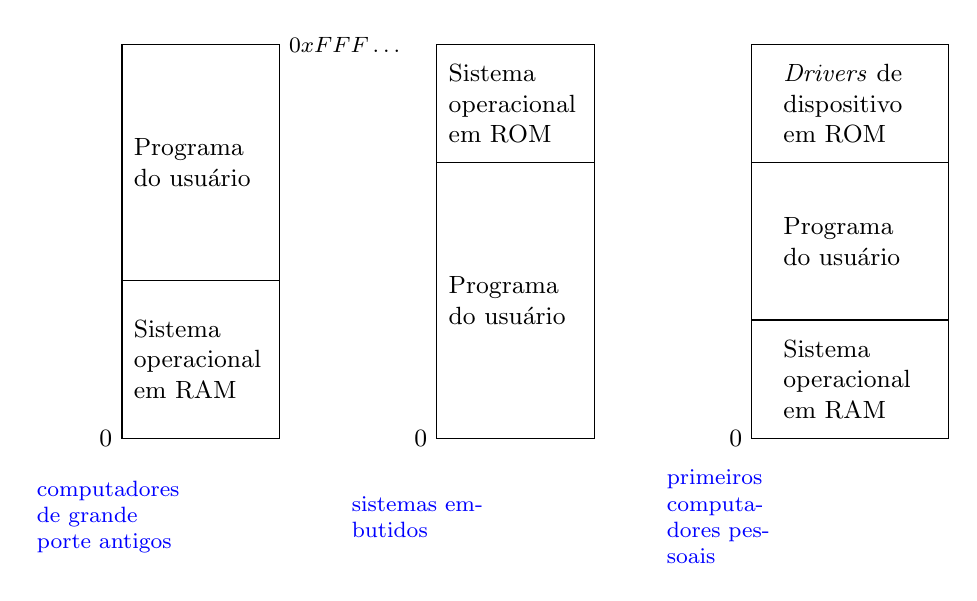
\begin{tikzpicture}
[mytext/.style={midway,text width=1.7cm,font=\small},
mycaption/.style={color=blue,anchor=east,text width=1.75cm,font=\footnotesize}]

\draw<2-> (0,0) node[left] (a) {\small 0} rectangle (2,2) node[mytext]{Sistema operacional em RAM};
\draw<2-> (0,2) rectangle (2,5) node[mytext]{Programa do usuário} node[right]{\footnotesize $0xFFF\dots$};

\node<2> [mycaption,below of=a] {computadores de grande porte antigos};

\draw<3-> (4,0) node[left] (b) {\small 0} rectangle (6,3.5) node[mytext]{Programa do usuário};
\draw<3-> (4,3.5) rectangle (6,5) node[mytext]{Sistema operacional em ROM};
\node<3> [mycaption,below of=b] {sistemas embutidos};

\draw<4-> (8,0) node[left] (c) {\small 0} rectangle (10.5,1.5) node[mytext]{Sistema operacional em RAM};
\draw<4-> (8,1.5) rectangle (10.5,3.5) node[mytext]{Programa do usuário};
\draw<4-> (8,3.5) rectangle (10.5,5) node[mytext]{\textit{Drivers} de dispositivo em ROM};
\node<4> [mycaption,below of=c] {primeiros computadores pessoais};
\end{tikzpicture}
\end{frame}

\newcounter{poscounter}\setcounter{poscounter}{28}
\begin{frame}{Execução de múltiplos programas}
\begin{tikzpicture}
\tikzset{mylabel/.style={font=\footnotesize,above right},
ref/.style={font=\footnotesize,below right}}
\def\w{1.4}
\def\h{.4}
\foreach \i/\p/\rp in {0/0/32,1/4/36,2/8/40,3/12/44,4/16/48,5/20/52,6/24/56,7/28/60} {
\def\thelabel{}
\ifnum\i=0
\def\thelabel{JMP 24}
\else\ifnum\i=6
\def\thelabel{MOV}
\else\ifnum\i=7
\def\thelabel{ADD}
\fi
\fi
\fi
 \draw<1,3>[fill=blue!40] (0,\i*\h) node[mylabel]{\thelabel} rectangle (\w,\i*\h+\h) node[ref]{\p};
 
 \def\thelabelb{}
\ifnum\i=0
\def\thelabelb{JMP 28}
\else\ifnum\i=7
\def\thelabelb{CMP}
\fi\fi
 
 \addtocounter{poscounter}{\p}
 \draw<2,3>[fill=red!20] (0,3.25+\i*\h) node[mylabel]{\thelabelb} rectangle (\w,3.25+\i*\h+\h) node[ref]{\only<2>{\p}\only<3>{\rp}};
}

\path[->,>=latex,draw]  (-1,3.25) node[left,draw]{32} -- (-0.1,3.25);

\end{tikzpicture}

\end{frame}


